Nektar++ is an open-source software package that uses spectral/hp element method to solve partial differential equations (PDEs). The solvers in the package support PDEs that can be applied to a wide range of areas such as fluid dynamics, structural dynamics and electrophysiology. The demand for low computational cost in almost all industries urges engineers to minimise computation time while maintaining a guaranteed level of accuracy. Compared to the traditional finite element method, spectral/$hp$ element method improves solution accuracy by refining both element size ($h$) and polynomial order ($p$). Previous studies have shown that the so-called $hp$-refinement converges at an exponential rate, making it more efficient than relying solely on $h$-type or $p$-type refinement \cite{RefWorks:karniadakis2005spectral/hp}. However, increasing both $h$-type and $p$-type refinement comes at the cost of increased computation time at varying rates. Consequently, determining the optimal combination of $hp$ is non-trivial. Furthermore, the optimal $hp$ combination is sensitive to the mathematical coefficients in the PDE and changes with the type of PDE to be solved. In addition to polynomial order and mesh element size, the discretisation is governed by a rich set of parameters. The choice of quadrature point distribution is one of them that could impact the accuracy and runtime of the solution. For example, misalignment in unstructured triangular elements and interpolation error can result in poor simulation quality in capturing regular geometries, such as a straight wavefront. In such cases, increasing the polynomial order with Gaussian quadrature point distribution may not improve the solution quality efficiently, due to the computation power not being distributed evenly. An alternative approach could involve using electrostatic point distribution which may offer better performance.
\par
This paper explores the optimal $hp$ combination and compares the performance of Gaussian and electrostatic quadrature point distributions for solving two-dimensional reaction-diffusion PDEs using high-order spectral/hp element method. Note that electrostatic distribution is also referred to as nodal distribution and both terms are used interchangeably in this paper. The CardiacEPSolver in Nektar++ was used to solve the monodomain equation as an example, with polynomial order ranging from 2 to 15 at varying mesh sizes on a rectangular domain. A visualisation of the example problem is shown in Figure \ref{domain}. The aim of this paper is to assist Nektar++ users in selecting optimal parameters for using the CardiacEPSolver. 
\par
The setup of the example problem and the experimental method are described in Section 2. Results and findings are presented and limitations are discussed in Section 3 and Section 4. Finally, advice on tuning parameters for the CardiacEPSolver is summarised in Section 5.
\begin{figure}[hb!]
    \centering
    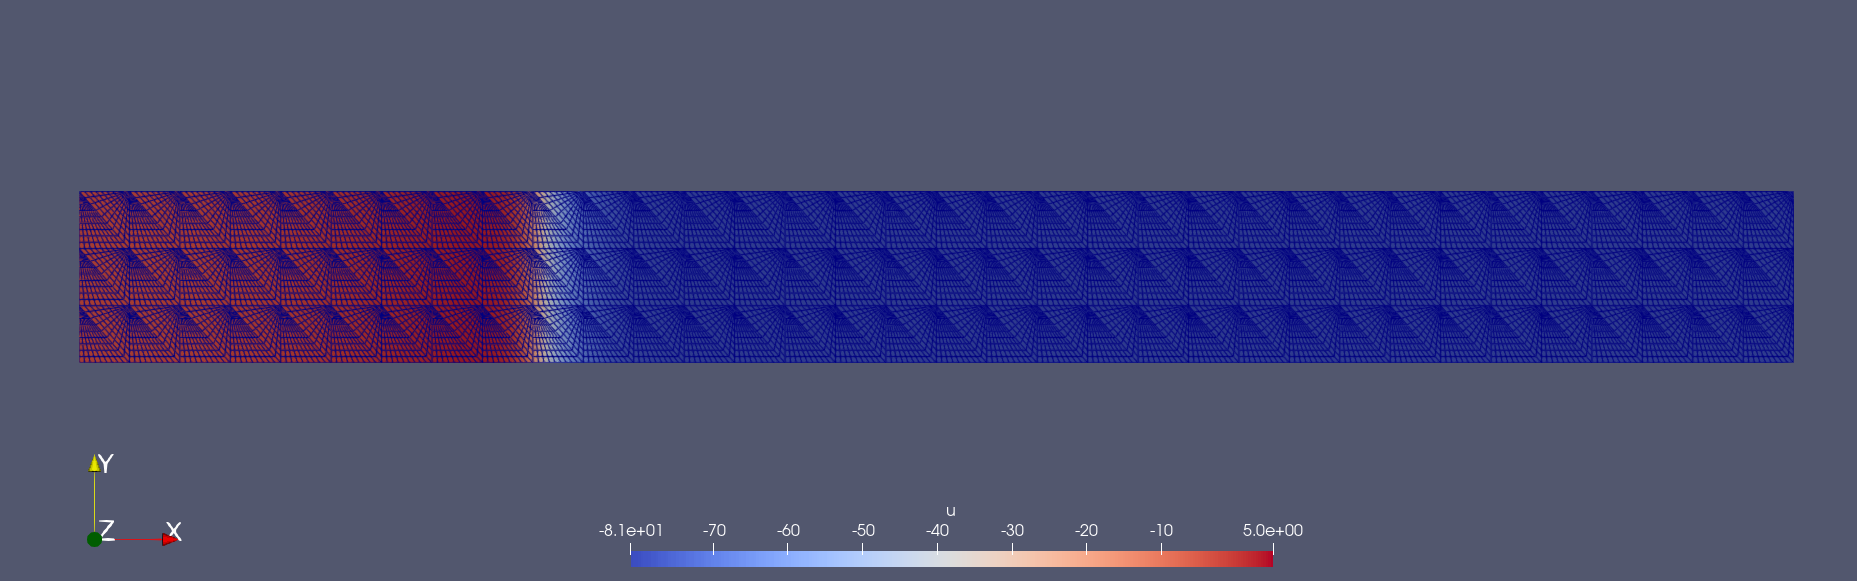
\includegraphics[width=0.7\linewidth]{figs/domain.png}
    \caption{Visualisation (in ParaView 5.11.0) of the solution to the monodomain equation on a rectangular domain showing action potential propagation. The colour bar indicates the voltage from -81.9V to 5V.}
    \label{domain}
\end{figure}
